%%%%%%%%%%%%%%%%%%%%%%%%%%%%%%%%%%%%%%%%%%%%%%%%%%%%%%%%%%%%%%%%%%%%%%%%%%%%
% FILE    : main.tex
% SUBJECT : Master document for the TISSEC 2014 paper.
% AUTHOR  : (C) Copyright 2014 by Peter C. Chapin and Christan Skalka
%
%%%%%%%%%%%%%%%%%%%%%%%%%%%%%%%%%%%%%%%%%%%%%%%%%%%%%%%%%%%%%%%%%%%%%%%%%%%%

\documentclass[prodmode,acmtissec]{acmsmall}

% --------
% Packages
% --------
\usepackage{fancyvrb}
\usepackage{stmaryrd}
\usepackage[english]{fp-autoref}
\usepackage{fp-frame}
\usepackage{soul}
\usepackage{mathpartir}
\usepackage{comment}
\usepackage{url}

% ------
% Macros
% ------
\newtheorem{condition}{Condition}[section]
\newtheorem{definition}{Definition}[section]
\newtheorem{theorem}{Theorem}[section]
\newtheorem{lemma}{Lemma}[section]
\newtheorem{corollary}{Corollary}[section]
\newtheorem{example}{Example}[section]
\newtheorem{proposition}{Proposition}[section]

\newcommand{\code}[1]{\texttt{\small #1}}
\newcommand{\filename}[1]{\texttt{#1}}
\newcommand{\newterm}[1]{\textit{#1}}

\long\def\cnote#1{\marginpar{CS}{\small \ \ $\langle\langle\langle$\
{#1 - CS}\
    $\rangle\rangle\rangle$\ \ }} 
\long\def\pnote#1{\marginpar{PC}{\small \ \ $\langle\langle\langle$\
{#1 - PC}\
    $\rangle\rangle\rangle$\ \ }} 


% -----
% Figures made Chris' way 
% -----
\newcommand{\snowcloudfig}
{
\begin{fpfig}[t]
{A Snowcloud Sensor Node (L,C) and Harvester Device (R).}
{figure-snowcloud}
\vspace{3mm}
\begin{center}
\begin{tabular}{ccc}
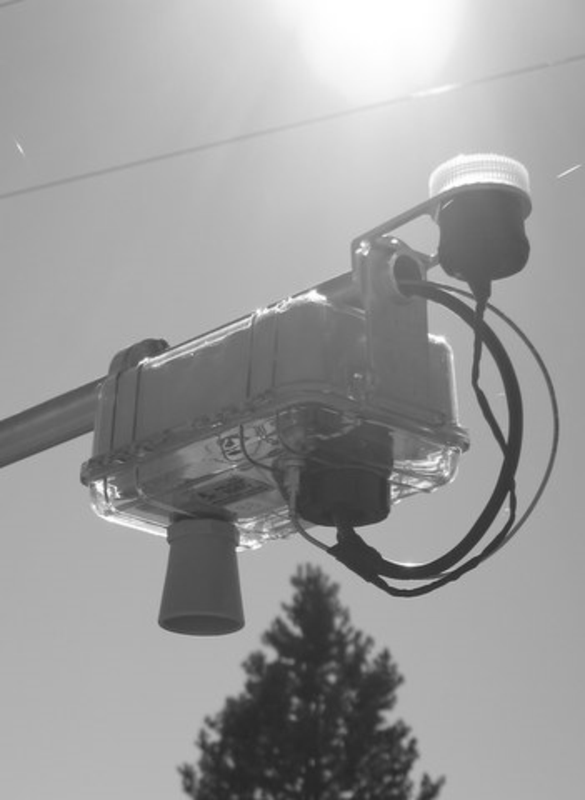
\includegraphics[scale=.35]{brainbox}
& 
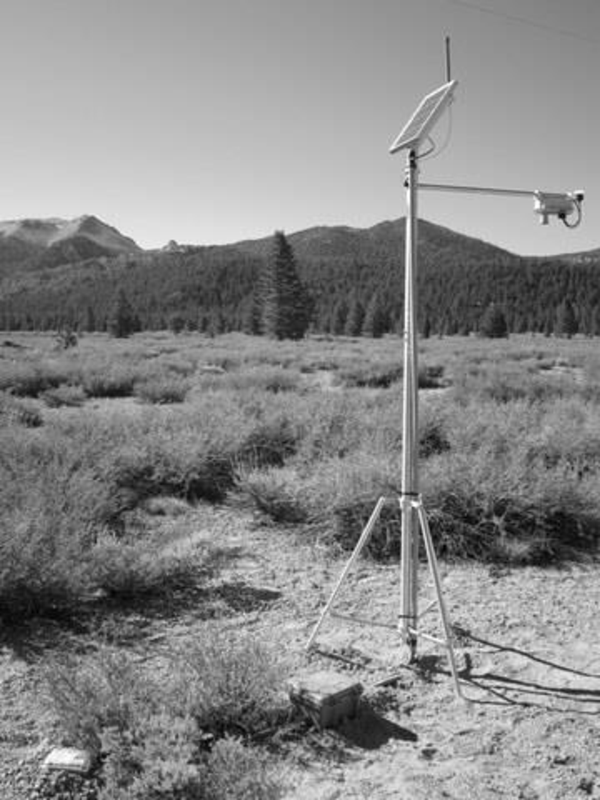
\includegraphics[scale=.35]{tower} 
&
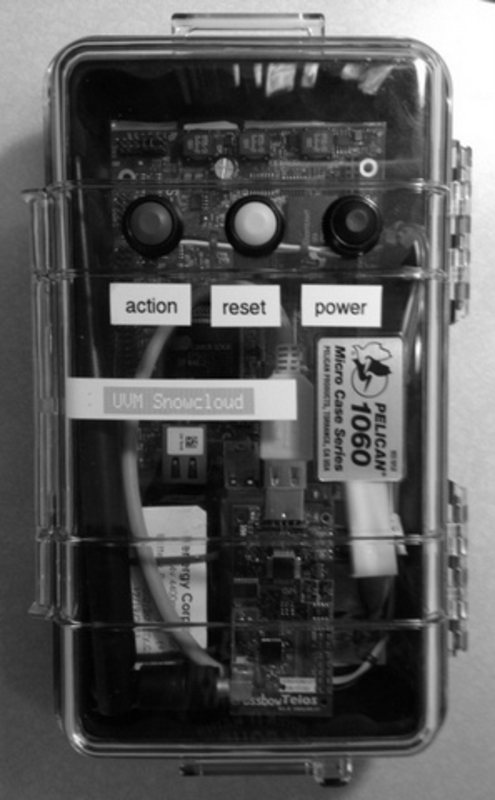
\includegraphics[scale=.35]{harvester} 
\end{tabular}
\end{center}
\end{fpfig}
}


% To be filled in after the paper is accepted.
%\acmVolume{V}
%\acmNumber{N}
%\acmArticle{A}
%\acmYear{YYYY}
%\acmMonth{0}

\markboth{P. Chapin and C. Skalka}{RPC Authorization in Sensor Networks}

% Title portion
\title{SpartanRPC: Remote Procedure Call Authorization in Wireless Sensor Networks}
\author{PETER CHAPIN and CHRISTIAN SKALKA \affil{University of Vermont}}

\begin{abstract}
  We describe SpartanRPC, a secure middleware technology that supports
  cooperation between distinct security domains in wireless sensor
  networks. SpartanRPC extends nesC to provide a link-layer remote
  procedure call (RPC) mechanism, along with an enhancement of
  configuration wirings that allow specification of remote, dynamic
  endpoints. RPC invocation is secured via an authorization logic that
  enables servers to specify access policies, and requires clients to
  prove authorization. This mechanism is implemented using a
  combination of symmetric and public key cryptography. We report on
  benchmark testing of a prototype implementation, and on an
  application of the framework that supports secure collaborative use
  and administration of an existing WSN data gathering system.
\end{abstract}

\category{D.3.4}{Programming Languages}{Processors}[Compilers \and
Run-time environments]
\category{C.3}{Computer Systems Organization}{Special-Purpose and
  Application-Based Systems}[Real-time and embedded systems]
\category{C.2.4}{Computer-Communication Networks}{Distributed
  Systems}[Client/server]

\terms{Security, Languages}

\keywords{remote procedure call, sensor networks, trust management}

\acmformat{Peter Chapin and Christian Skalka. 2014. SpartanRPC: Remote
  Procedure Call Authorization in Wireless Sensor Networks}

\begin{document}

\begin{bottomstuff}
  Christian Skalka’s work was supported by a grant from the Air Force
  Office of Scientific Research Young Investigator Program (AFOSR YIP).

  Author's addresses: P. Chapin, (Current address) Computer Information
  Systems Department, Vermont Technical College; C. Skalka, Computer
  Science Department, University of Vermont.
\end{bottomstuff}

\maketitle

% ----------------
% Document content
% ----------------
\section{Introduction}
\label{section-intro}

As WSN technology becomes more ubiquitous applications of overlapping yet independently
controlled sensor networks will begin to appear. Networks from cooperating but distinct security
domains may wish to use each other's nodes to increase the resolution, spacial coverage, or
lifespan of certain sensing or control functions. For example, assume that two distinct networks
are deployed to the same space such that nodes from both networks can communicate with each
other. While the primary purpose of the two networks might be independent, their administrators
might nevertheless agree to collaborate on certain supporting functionality such as data
collection and analysis.

Although in some cases data collected by each security domain could be shared off-network,
perhaps via Internet connected gateways, certain advantages could be gained by enabling
in-network interactions. For example if one network is partitioned due to a failed node, the
separated partitions might be able to continue communicating by routing their messages over a
cooperating network's nodes.

In situations where low latency is important, such as with time synchronization protocols
\cite{ganeriwal-kumar-srivastava-2003}, in-network interactions between independent, cooperating
WSNs would be more effective than attempting to synchronize two networks via long distance
Internet links. Tracking applications \cite{brooks-ramanathan-sayeed-2003} could also benefit
from in-network interactions between cooperating networks. Handing off tracking information from
one network to another via an Internet link would require activating a potentially large number
of nodes in each network in order to send information to their respective gateways. This creates
power consumption concerns. Other potential applications where in-network interactions could
play a role include secure routing protocols in heterogeneous trust environments
\cite{senroute-ahnj03}, transport and network layer protocols \cite{perillo-heinzelman-2005},
and even mote-based web servers supporting secure channels \cite{1049776}.

High level applications can also benefit from in-network interactions between cooperating WSNs.
For example, the use of WSNs to facilitate emergency care in disaster situations has been
described \cite{citeulike:4460555,1038146}. While this previous work has focused on WSNs in a
single security domain, it is likely that multiple domains would be in use during many
emergencies as first responders from different organizations or different political
jurisdictions work together. In those cases it is not realistic to assume that each domain would
have Internet connectivity; the disaster site might be too remote or the supporting network
infrastructure might be non-functional. Direct interaction between the WSNs of cooperating
domains becomes an effective way for them to share information.

In this paper we describe novel middleware technology to support WSN applications in this
setting. Our system, which we call SpartanRPC, provides a new form of link-layer RPC as a
natural extension of the nesC programming model, and \emph{language based authorization} based
on symmetric-key cryptography. As other authors have observed \cite{may-tinyrpc-2007}, RPC is an
appropriate abstraction for node services on the network and supports whole-network
(vs.~node-specific) programming. We further observe that RPC allows nodes to provide flexible,
modular services without the need for reprogramming, a kind of ``micro web services.''
\emph{Secure} RPC is also clearly desirable in a heterogeneous trust environment.

\subsection{Overview and Contributions}

Previous related work illustrates interest in and useful applications of RPC in a WSN context.
For example, the Marionette system uses network layer RPC for remote (PC-based) analysis and
debugging of WSNs \cite{whitehouse-marionette-2006}. The Fleck operating system provides a small
pre-defined set of RPC services for WSN applications, while the secFleck system extends this
with a form a secure RPC \cite{hu-secfleck-2009}. SpartanRPC differs from these systems in that
it extends the nesC programming language to allow programmer definition (unlike secFleck) of
secure RPC services that can be accessed by nodes within the network itself (unlike Marionette).
Our system is similar to and inspired by TinyRPC \cite{may-tinyrpc-2007}, except the latter does
not provide security and has a different semantics that is not as expressive and flexible as our
approach.

Major contributions of our work include an RPC design that is consistent with existing nesC
semantics, including an asynchronous ``task-like'' conception of RPC and \emph{dynamic wires} as
a natural extension of configuration wirings to allow flexibility in remote communication. We
also provide a mechanism for fine-grained RPC authorization. Finally we created an
implementation of SpartanRPC \cite{sprocket} from which we obtained empirical results showing
that SpartanRPC features are not onerous in terms of additional space and energy consumption.
   
A primary goal of the SpartanRPC design is to provide RPC capabilities as transparently as
possible. This means at least that the low-level communication details should be hidden from the
user. Beyond that, it means that RPC features should be provided in a manner that fits in with
existing nesC semantics.

\paragraph{Asynchronous Execution Model} In nesC a \emph{command} is a synchronous unit of
control; when one is called, it is pushed onto the call stack and the current continuation waits
for the command to complete and yield a result. In contrast, when a \emph{task} is posted it is
placed in a queue for execution at some future time, and the calling context continues
immediately. We propose a task-like mechanism for RPC invocation, that allows \emph{remote
  postings}; in this our approach differs from TinyRPC that envisioned RPC as a form of command
\cite{may-tinyrpc-2007}. However, our mechanism differs from tasks in two important ways: first,
we allow arguments to be passed in RPC calls, and second, the module that posts an ordinary task
must define it, whereas we want to allow modules to execute functionality defined non-locally.
We therefore introduce the \emph{duty} mechanism. Duties may be posted like a task, but passed
arguments and provided by modules for posting by other (possibly non-local) modules. Duties are
discussed in Sect.~\ref{section-duties}.

\paragraph{Dynamic Wires} The SpartanRPC design provides a minimalist extension of configuration
wiring syntax with abstractions for remote communication. In our system components can provide
remotable interfaces, and in configuration definitions these interfaces can be wired to locally
or non-locally. However, wirings to remote interfaces must specify the host of the wired-to
component, and our syntax requires the user to provide an inherently dynamic definition of
endpoint hosts to allow fan-out wirings that can change at run-time. Since SpartanRPC works at
the link layer, we believe this flexibility is fundamental in a general WSN setting where
neighborhoods can be expected to change frequently due to node repositioning, failure, or
changes in radio signal strengths. Dynamic wires are discussed more in
Sect.~\ref{section-dynamic-wires}.

\paragraph{Fine-Grained Authorization Policies} Research on WSN security has addressed secure
routing \cite{senroute-ahnj03}, link layer security \cite{karlog-tinysec-2004}, cryptography
\cite{bertoni-2006} and key distribution \cite{camtepe-bulent-05}, and hardware issues
\cite{perrig-2004}. This previous work has established a strong low-level foundation for
security in WSNs. We believe that secure link-layer RPC is an appealing middleware solution in
WSNs because it allows programmatic specification of previously ad-hoc network-level behavior,
while imposing relatively small syntactic and efficiency overhead. SpartanRPC also allows
multiple symmetric keys to be used to protect multiple security domains within a network in a
simple and usable manner. Our security mechanism is discussed in more detail in
Sect.~\ref{section-security-extensions}.

\section{Duties and Remotability}
\label{section-duties}

Because of the slow, unreliable nature of wireless communications we believe it is unrealistic
for RPC services in WSNs to be synchronous. Instead we believe that the semantics of tasks are
closer to being a correct abstraction. They are not quite right however, as RPC services will
typically require arguments to be passed, and while the poster of a task defines it, an RPC
service invokes remotely defined functionality. We therefore define a new RPC abstraction called
a \emph{duty}.

\subsection{Syntax and Semantics}
\label{section-duties-syntax}

Duties are declared in interfaces and syntactically resemble command declarations. Instead of
using the reserved word \code{command} the new reserved word \code{duty} is used. Duties are
allowed to take parameters (with restrictions as discussed below) but must return the type
\code{void}. For example the following interface describes an RPC service for remotely flashing
a mote LED:
\begin{Verbatim}
interface LEDControl {
    duty void setLeds(uint8_t ctl);
}
\end{Verbatim}

Duties are defined in modules in a manner similar to the way tasks, commands, or events are
defined. The reserved word \code{duty} is again used on the definition. Like commands and events
the name of the duty is qualified by the name of the interface in which it is declared.
Including a duty in an interface definition automatically implies that the interface can be
remotely invoked, or is \emph{remotable} in the sense formalized in
Sect.~\ref{section-remotable}. Any remotable interface provided by a component must be specified
as \code{remote} in its provides specification, for example:
\begin{Verbatim}
module LEDControllerC {
    provides remote interface LEDControl;
}
implementation {
    duty void LEDControl.setLeds(uint8_t ctl)
    { ... }
}
\end{Verbatim}

A module on the client node that wishes to use a remotable interface simply posts the duty in
the same manner as tasks are posted. The use of \code{post} emphasizes the asynchronous nature
of the invocation.
\begin{Verbatim}
module LoggerC {
    uses interface LEDControl;
}
implementation {
    ...
    post LEDControl.setLeds(42);
}
\end{Verbatim}

Note that the standard component semantics of nesC provide here a natural abstraction of
``where'' the RPC call goes, just as e.g.~a normal command invocation will go through a
component interface that is disconnected from its implementation. Like a normal command
invocation, configuration wirings determine where duty control flows. However, in SpartanRPC
duty invocation control may flow to a component residing on a different network node. The
invoking module must be connected to the remote modules by way of a dynamic wire as described in
Sect.~\ref{section-dynamic-wires}.

When a duty is posted by a client node it may run at some time in the future on the server node.
The client node continues at once without waiting for the duty to start, i.e.~duty postings are
asynchronous in the same manner that tasks are. Once posted the client has no direct way to
determine the status of the duty. Also, due to the unreliability of the network a posted duty
may not run at all.

It is possible for a duty to be posted multiple times by a client or by multiple clients.
Because duties are implemented as nesC tasks as discussed in Sect.~\ref{section-implementation},
any posts of a particular duty received by a node while a previous post of that duty is pending
are lost. However, this does not introduce any new problems because duty execution is not
guaranteed in any case.

\subsection{Remotable Interfaces}
\label{section-remotable}

We impose certain requirements on RPC service definitions for ease of implementation. First,
since WSN nodes do not share state we disallow passing references to duties---such a reference
would be meaningless on the receiving node. Thus we define remotable types:
\begin{definition}A type is \emph{remotable} iff it satisfies the following inductive
  definition: The nesC built-in arithmetic types, including enumeration types, are remotable,
  and arrays of remotable types and structures containing remotable types are remotable.
\end{definition}
Since a remotable interface describes RPC services, we require that they specify duties taking
only arguments of remotable type; also, remotable interfaces can only contain duties, to ensure
meaningful remote usage.
\begin{definition}
  An interface is \emph{remotable} iff it only provides duties whose argument types are
  remotable.
\end{definition}

\section{Dynamic Wires}
\label{section-dynamic-wires}

In an ordinary nesC program the ``wiring'' between components as defined
by configurations is entirely static. The nesC compiler arranges for all
connections, and at run time the code invoked by each called command or
signaled event is predetermined.

In a remote procedure call system for wireless networks this static
arrangement is insufficient. A node can not, in general, know its
neighbors at compilation time but rather must discover this information
after deployment. In addition, the volatility of wireless links and of
the nodes themselves means that a given node's set of neighbors will
change over time. In this section we discuss the facility in SpartanRPC
to allow \emph{dynamic wirings} for specifying control flow from duty
invocation to duty implementation.

\subsection{Component IDs, Component Managers}
\label{section-componentmanager}

We begin by discussing how remote components are identified for wiring.
In order to uniquely identify components on the network, remotable
components are specified via a two-element structure called a
\code{component\_id} defined on the left side of
\autoref{figure-componentmanager}. The \code{node\_id} member is the
same node ID used by TinyOS and is set when the node is programmed
during deployment. The local ID member is an arbitrary value defined by
the programmer of the server node. Only components that are visible
remotely need to have ID values assigned, however, the ID values must be
unique \emph{on the node}. The \code{component\_set} structure defined
on the right side of \autoref{figure-componentmanager} wraps an
arbitrary array of \code{component\_id} values.
 
\begin{figure}[!t]
\begin{textbox}{4in}
\begin{minipage}[t]{1.75in}
\begin{Verbatim}[fontsize=\small]
    typedef struct {
        uint16_t node_id;
        uint8_t  local_id;
    } component_id;
\end{Verbatim}
\end{minipage}
\hfill
\begin{minipage}[t]{1.75in}
\begin{Verbatim}[fontsize=\small]
typedef struct {
    int count;
    component_id *ids;
} component_set;
\end{Verbatim}
\end{minipage}
\\
\centering
\begin{minipage}[t]{5.8in}
\vspace{1.5em}
\begin{Verbatim}[fontsize=\small]
interface ComponentManager { command component_set elements(); }
\end{Verbatim}
\end{minipage}
\end{textbox}
\caption{Component Manager Interface and Type Definitions}
\label{figure-componentmanager}
\end{figure}

A \emph{component manager} is a component that provides the
\code{ComponentManager} interface defined at the bottom of
\autoref{figure-componentmanager}. It dynamically specifies a set of
component IDs that ultimately serve as dynamic wiring endpoints. An
example component manager is discussed in detail
\autoref{section-example}.

As a simple example, consider the component manager
\code{RemoteSelectorC} as shown in
\autoref{figure-example-componentmanager}. This component manager always
returns a component set containing a single component. The special
SpartanRPC broadcast node ID is used (\code{0xFFFF}) indicating that all
neighbors should be the target of the dynamic wire. The component ID on
the neighbors is specified as $1$ in this example. In a more complex
example the component manager would compute the component set each time
the dynamic wire is used, filling in an array of component IDs based on
information gathered earlier.

\begin{figure}[!t]
\begin{textbox}{4.0in}
\begin{Verbatim}[fontsize=\small]
module RemoteSelectorC { provides interface ComponentManager; }
implementation {
    component_id  broadcast  = { 0xFFFF, 1 };
    component_set broadcast_set = { 1, &broadcast };

    command component_set ComponentManager.elements() {
        return broadcast_set;
    }
}
\end{Verbatim}
\end{textbox}
\caption{Example Component Manager}
\label{figure-example-componentmanager}
\end{figure}

\subsection{Syntax and Semantics}
\label{section-wiringsyntax}

In SpartanRPC we extend the syntax and semantics of nesC to allow the
target of a connection to be dynamically specified by a component
manager. The syntax of wirings, or connections, is extended as follows:

\begin{lrbox}{\savebigbox}
\begin{minipage}{4.3in}
\vspace{0.6em}
\begin{Verbatim}[fontsize=\small]
        connection ::= endpoint '->' dynamic_endpoint
  dynamic_endpoint ::= '[' IDENTIFIER ']' ('.' IDENTIFIER)?
\end{Verbatim}
\vspace{0.3em}
\end{minipage}
\end{lrbox}
\centerline{\usebox{\savebigbox}}

Given a dynamic wiring of the form \code{C.I -> [M].I}, we informally
summarize its semantics as follows. First, we statically require that
\code{M} be a component providing the \code{ComponentManager} interface,
and that \code{I} be a remotable interface. At run time, if control
flows across this wire via posting of some duty \code{I.d} within
component \code{C}, the command \code{elements} in \code{M} is called to
obtain a set of component IDs. The duties \code{I.d} provided by the
specified remote components will then be posted on their respective
nodes via an underlying link layer communication, the details of which
are hidden from the programmer. Thus, duties can only be posted on
neighbors. Note that since this call to \code{elements} may return more
than one component ID, this is a sort of fan-out wiring.

For example, the programmer could wire the \code{LoggerC} component
mentioned in \autoref{figure-duty-usage} to LED controller components on
a dynamically changing subset of neighbors using a configuration such
as:
\begin{Verbatim}[fontsize=\small, commandchars=\\\{\}]
\centerline{LoggerC.LEDControl -> [RemoteSelectorC];}
\end{Verbatim}

The server's configuration does not need to wire anything to the remote
interface explicitly.

\subsection{Callbacks and First-Class IDs}

We assume that the component IDs for well known services will be agreed
upon ahead of time by a social process outside of our system. By
broadcasting to a well known component ID, a node can use services on
neighboring nodes without knowing their node IDs.

If a node expects a reply from a service that it invokes, the invoking
node must set up a component with a suitable remote interface to receive
the service's result. In SpartanRPC remote invocations can only transmit
information in one direction. Bidirectional data flow requires separate
dynamic wires. This design provides a natural ``split-phase'' semantic
in which the invoker of a service can continue executing while waiting
for the result of that service. For example, a service might require the
client to provide the node ID and component ID of the component that
will receive the service result as arguments to the service invocation.
The server could store those values for use by a server-side component
manager. It is permitted for a component to be its own component manager
making it easy for a service to return a result by posting the
appropriate duty.

% For example, assume that the LED controller on the server returns the
% old state of the LEDs whenever the LED value is changed. The server
% configuration would include an appropriate dynamic wire as follows
%
% \begin{Verbatim}[commandchars=\\\{\}, fontsize=\small]
% \centerline{LEDControllerC.LEDResult -> [LEDControllerC];}
% \end{Verbatim}
%
% The client must provide the LEDResult interface remotely to receive
% this result. In this example the \code{LEDControllerC} component is
% its own component manager. This makes it easy for the \code{elements}
% command to access global data that was recorded inside
% \code{LEDControllerC} when the service it provides was previously
% invoked. This is a common SpartanRPC idiom.

\section{Security Policy Specification and Program Logic}
\label{section-security-extensions}

In this section we discuss how to extend the language setting described
previously with security features. The goal is a language framework
where RPC services require authorization for use, and where
authorization policies support collaboration between multiple security
domains. To this end we adapt a distributed trust management system
\cite{chapin-skalka-wang-acmcs08} for policy specification. This system
secures WSN application programming by way of the SpartanRPC API.

\subsection{Security Policy Language}

Authorization in trust management systems is more expressive than in
traditional access control schemes such as access control lists or role
based access control (RBAC) \cite{Sandhu:RBACM}. In these simpler
models, access is based on identities of principals. But in the
distributed scenarios we are considering here, creating a single local
database of all potential requesters is untenable. Where there are
multiple domains of administrative control, no single authorizer can
have direct knowledge of all users of the system. Furthermore, in highly
dynamic and volatile environments, no single entity in-network can be
expected to keep pace with changes in an authoritative manner. Finally,
basing authorization purely on identity is not a sufficiently expressive
or flexible approach, since security in modern distributed systems
utilizes more sophisticated features (e.g.~delegation). These problems
are addressed by the use of trust management systems such as the \RT\
framework \cite{Li:DRBTMF}. We use the system $\RT_0$ in this
foundational presentation due to its simplicity, but other $\RT$
variants \cite{Li:DCDTM,Li:RRBTMF} could be adapted.

Like other trust management systems such as SPKI/SDSI \cite{RFC-2693},
\RT\ represents principals as public keys and does not attempt to
formalize the connection between a key and an individual. The \RT\
literature usually refers to principals as \newterm{entities}. \RT\
allows each entity to define \emph{roles} in a name space that is local
to that entity. An authorizer associates permissions with a particular
role; to access a resource a requester must prove membership in the
role. In this way \RT\ provides a form of role based access control.

To define a role, an entity issues credentials that specify the role's
membership. Some of these credentials may be a part of private policy,
others may be signed by the issuer and made publicly available as
certificates. The overall membership of a role is taken as the union of
the memberships specified by all known defining credentials.

Let $A, B, C, \ldots$ range over entities and let $r, s, t, \ldots$
range over role names. A role $r$ local to an entity $A$ is denoted by
$A.r$. \RT\ credentials are of the form $\cred{A.r}{f}$, where $f$ can
take on one of four forms to obtain one of four credential types:
\begin{longenum}

\item $\cred{A.r}{E}$. This form asserts that entity $E$ is a member of
  role $A.r$.

\item $\cred{A.r}{B.s}$. This form asserts that all members of role
  $B.s$ are members of role $A.r$. Credentials of this form can be used
  to delegate authority over the membership of a role to another entity.

\item $\cred{A.r}{B.s.t}$. This form asserts that for each member $E$ of
  $B.s$, all members of role $E.t$ are members of role $A.r$.
  Credentials of this form can be used to delegate authority over the
  membership of a role to all entities that have the attribute
  represented by $B.s$. The expression $B.s.t$ is called a \emph{linked
    role}.

\item $\cred{A.r}{q_1 \cap \cdots \cap q_n}$. Where the $q_i$ are
  qualified role names such as $B.s$. This form asserts that each entity
  that is a member of all roles $q_1,\ldots, q_n$ is also a member of
  role $A.r$. The expression $q_1 \cap \cdots \cap q_n$ is called an
  \emph{intersection role}. In our implementation only two constituent
  roles $q_1$ and $q_2$ are allowed in an intersection role. This does
  not limit expressivity since intermediate roles can be introduced as
  necessary to handle larger intersections.

\end{longenum}
For all credential forms $\cred{A.r}{f}$, the principal $A$ is called
the \emph{issuer} of the credential. An example credential set is
presented and discussed in \autoref{section-snowcloud}.

The formal semantics of \RT\ can be expressed in terms of \datalog\
\cite{Li:DRBTMF}. The translation of \RT\ credentials to \datalog\
requires only a single relation \textit{isMember} to assert when a
particular entity is a member of a particular role. A type (1)
credential, called a \newterm{membership credential}, is translated into
\datalog\ simply as a fact. For example the credential $\cred{A.r}{E}$
becomes the fact $\textit{isMember}(E, A, r)$. The other three
credential types are translated into \datalog\ rules. For example, the
type (3) credential $\cred{A.r}{B.s.t}$ becomes the following \datalog\
rule:\footnote{Logical variables are shown prefixed with `\textit{?}'}

\begin{displaymath}
\textit{isMember}(\textit{?x}, A, r) \leftarrow
  \textit{isMember}(\textit{?y}, B, s),
  \textit{isMember}(\textit{?x}, \textit{?y}, t).
\end{displaymath}

The meaning of an \RT\ credential $\semantics{C}$ is the \datalog\ fact
or rule to which it translates. Let $\creds$ be a set of \RT\
credentials split into two disjoint subsets $\creds = \creds_f \amalg
\creds_r$ where $\creds_f$ is the set of all membership credentials. The
meaning of $\creds$, which we denote as $\semantics{\creds}$, is the
minimum model of the \datalog\ program $\semantics{\creds_r}$ using
$\semantics{\creds_f}$ as input \cite{Abiteboul:FD}. The authorizer
associates an access permission with a particular role, say $A.g$, that
we call the \newterm{governing role}. Hence we formally define
authorization in a given credential environment $\creds$ as follows:

\begin{definition}
  Given a credential set $\creds$, entities $A$ and $E$, and role $g$,
  \emph{$E$ is authorized for $A.g$ in $\creds$}, denoted $\creds \vdash
  E \in A.g$, if and only if $\textit{isMember}(E, A, g)$ is in
  $\semantics{\creds}$.
\end{definition}

One appealing characteristic of the $RT_0$ trust management system is
monotonicity. Negative credentials that explicitly remove entities from
roles are not supported. Consequently if an authorizer has incomplete
information she might deny access that would otherwise be granted, but
she will never grant access that should have been denied. This property
is essential in a WSN context where the unreliability of wireless
communication together with the limited memory resources of sensor nodes
make it impossible to \emph{guarantee} complete information about all
roles.

Our system requires the requester to provide all necessary credentials
using some external means to obtain them. Methods for doing, for
example, distributed credential chain discovery have been described
\cite{Li:DCDTM} but we feel they would be prohibitively expensive in a
WSN context. The best approach for collecting a complete set of
credentials may be application specific, and thus we regard it as
outside the scope of this work.

The use of $RT_0$ means that principles cannot switch to roles of lesser
privilege, as is often desirable in accordance with the principle of
least privilege. However, variants of \RT\ are available that support
switching to less privileged roles \cite{Li:RRBTMF}, and that could be
used in SpartanRPC instead of $RT_0$. Also techniques for supporting
certificate revocation in an \RT-style trust management framework have
been explored \cite{lbi-fc01}.

\begin{comment}
  \paragraph{ECC Public Key Cryptography} Trust management systems such
  as \RT\ depend on public key cryptography. Distributed certificates
  are protected with digital signatures made using the issuer's private
  key. Furthermore public key cryptography is used to authenticate
  message senders to ensure that the entity requesting a service is the
  entity it claims to be. However, public key cryptography is
  computationally expensive and this presents a problem for limited
  devices such as wireless sensor network nodes.

  The on-node cryptographic computations required by our system are
  digital signature verification, session key negotiation using
  Diffie-Hellman key exchange, and message authentication code (MAC)
  computation using a session key. Of these three operations the first
  two involve complex public key cryptography. The MAC computation
  occurs much more frequently but is much cheaper since it uses hardware
  accelerated symmetric key cryptography. In fact, the motivation behind
  creating session keys is to avoid public key operations for every
  message.

  Although the RSA public key cryptosystem has been implemented on
  sensor nodes \cite{Gura04comparingelliptic,wang-2006}, the resource
  consumption required to do so is considerable. However, the
  feasibility of using elliptic curve public key cryptosystems (ECC) on
  such platforms has been repeatedly demonstrated
  \cite{1049776,Malan:2008:IPI:1387663.1387668,Liu-Peng-TinyECC-2008,Szczechowiak:2008:NTL:1786014.1786040}.
  Hardware implementations of ECC for resource limited devices have also
  been demonstrated \cite{kumar-2006,4604657}.

  ECC can achieve much higher security for a given number of key bits
  saving memory and network bandwidth relative to other public key
  cryptosystems. In our implementation, described in detail in
  \autoref{section-implementation}, we use 160 bit ECC keys, providing a
  security similar to 1024 bit RSA keys \cite{lenstra-verheul-2001}. We
  believe this is a reasonable level of security for the anticipated
  applications.
\end{comment}

\subsection{Program Logic}

Our authorization model can be viewed as a client-server interaction;
respective sides of the interaction protocol are summarized separately
as follows.

\subsubsection{RPC Server Side Logic}
\label{section-rpc-server-side}

RPC service providers establish policy by assigning governing roles
$A.g$ to remote interface implementations. Service providers also
possess a set of assumed credentials $\creds$ which establish an
authorization environment by providing initial server side authorization
policy. As we will describe in detail, the set $\creds$ may grow as
additional credentials are communicated to servers. Finally, in the
presence of security, client invocations of any RPC service are not
anonymous, but are performed on behalf of some entity $B$, which must be
a member of the governing role $A.g$ to use the protected service.

In summary, access to an RPC level is allowed if and only if the
property $\creds \vdash B \in A.g$ holds, where:
\begin{itemize}
  \item $B$ is the identity of the RPC client
  \item $A.g$ is the governing role of the RPC service
  \item $\creds$ are the credentials known to the RPC host server
\end{itemize}
RPC service programmers specify governing roles as part of module
definitions---specifically at remote interface \texttt{provides}
clauses. Hence, governing roles are associated with interface
\emph{implementations}, not interfaces themselves. This allows
application flexibility, in that the same interface can be implemented
with various authorization levels within the same network. Syntax is as
follows:

\begin{Verbatim}[fontsize=\small, commandchars=\\\{\}]
\centerline{provides remote interface \textit{I} requires \textit{A.g}}
\end{Verbatim}

Note the minor modification to previously introduced syntax for remote
module definitions via the \texttt{requires} keyword.

\subsubsection{RPC Client Side Logic}
\label{section-rpc-client-side}

In order to use a secure remote module, RPC clients wire to it as for
unsecured modules (see \autoref{section-wiringsyntax}), but with two
additional capabilities: (1) the client specifies under what \RT\ entity
the invocations will be performed, and (2) the client may also specify
credentials in their possession which are to be activated for use in the
invocation. Syntax is as follows:

\begin{Verbatim}[fontsize=\small, commandchars=\\\{\}, codes={\catcode`*=3\catcode`!=8}]
\centerline{enable "*C!1, \ldots, C!n*" as "*B*" for C.I -> [M].J}
\end{Verbatim}

For any invocation made through this wiring the credentials $C_1,
\ldots, C_n$ will be remotely added to the RPC server's database for the
authorization decision, via a process detailed in
\autoref{section-implementation}. Note that these credentials \emph{need
  not establish authorization entirely by themselves}, rather they will
be \emph{added} to the server's existing credentials, all of which will
be used in the authorization decision. A special form of the
\code{enable} clause using \code{"*"} for the list of credentials is
also supported. This form indicates that all credentials known to the
client should be communicated to the server.

Each node is deployed with a collection of ECC key pairs, one for each
entity the node represents. When an invocation is made the entity $B$
mentioned in the \code{as} clause of the dynamic wire is used in the
request. The \code{as} clause is optional; if it is omitted a
distinguished \newterm{default entity} is used for the invocation.

% The reader will also note the syntax \texttt{assuming "$D_1, \ldots,
% D_k$"} above, which denotes the client's assumptions about credentials
% already known to the RPC server(s). Although this language does not
% have run-time relevance per se, its purpose is to allow static
% checking of enabled credentials on the client side. That is, the
% client possesses static knowledge of the governing role $A.r$ required
% to use modules provided as $[M].J$. \cnote{There is a problem here,
% how will the client know this? Note that this is a different matter
% than knowing about interfaces, which are ``constant''-- we have
% already allowed that different modules may implement interfaces at
% different security levels, so how do we ``keep track'' of them? It
% would be nice to resolve this, since static checking of this form is
% an appealing feature...} The system will statically verify the
% property $$C_1, \ldots, C_n, D_1, \ldots, D_k \vdash B \in A.r$$ and
% report an error in case the specified credentials are insufficient to
% establish authorization. Note that the client need not actually
% possess credentials $D_1, \ldots, D_K$ for this check to succeed;
% also, it may be the case that these credentials are not in fact known
% by the server, so that a successful check does not guarantee runtime
% authorization.

\begin{comment}
  \subsubsection{Example}
  \label{section-security-example}

  Suppose that an existing network deployment \code{NetA} is imaged with
  a component \code{SamplingRateC} which provides a means to control
  sampling rates through an interface \code{SamplingRate}. Further,
  since sampling rate modification is a sensitive operation, the network
  administrators require \code{NetA.control} authorization to use this
  component:

  \begin{lrbox}{\savebigbox}
  \begin{minipage}{5.0in}
  \vspace{0.6em}
  \begin{Verbatim}[fontsize=\small]
  module SamplingRateC {
      provides remote interface SamplingRate requires "NetA.control";
  }
  \end{Verbatim}
  \vspace{0.3em}
  \end{minipage}
  \end{lrbox}
  \centerline{\usebox{\savebigbox}}

  \noindent Any node supporting this component will transparently
  receive \RT\ credentials from neighboring nodes and attempt to use
  those credentials to establish that each client entity is a member of
  the \code{NetA.control} role in the formal sense described above.

  Suppose also that nodes in \code{NetA} are deployed with the credential

  \begin{displaymath}
  \code{NetA.control} \leftarrow \code{WSNAdmin.control}
  \end{displaymath}

  Here the role \code{WSNAdmin.control} is administered by some
  overarching network authority. However this authority need not be
  physically ``present'' in the network during operation. Instead the
  credential above represents \code{NetA}'s access control policy: any
  entity blessed by \code{WSNAdmin} as a controller can control
  \code{NetA}.

  Suppose further that another subnet, called \code{NetB}, wishes to
  modify the sampling rate of \code{NetA}. A node in \code{NetB} might
  be imaged with the following credentials, among possibly others:

  \begin{eqnarray}
  \code{WSNAdmin.control} & \leftarrow & \code{NetB.control} \\
  \code{NetB.control}     & \leftarrow & \code{NetB}
  \end{eqnarray}

  Note that credential (1) is issued by the \code{WSNAdmin} authority,
  while credential (2) is issued by \code{NetB}. Critically, direct
  communication with \code{NetA} authorities to obtain these credentials
  is unnecessary.

  In order to invoke this service the wiring as shown in
  \autoref{figure-secure-wire} could be made on the client side. Note
  the activation of the necessary credentials, as well as the
  specification of client identity as \code{NetB}.

  \begin{figure}[!t]
  \begin{textbox}{3.0in}
  \begin{Verbatim}[fontsize=\small]
  enable
    "WSNAdmin.control <- NetB.control, 
      NetB.control    <- NetB" as "NetB"
  for 
    ClientC.SamplingRate -> [RemoteSelectorC];
  \end{Verbatim}
  \end{textbox}
  \caption{Security Enabled Dynamic Wire}
  \label{figure-secure-wire}
  \end{figure}

\end{comment}

\section{Example: Secure Directed Diffusion}
\label{section-example}

To illustrate our language design we have implemented a secured version
of the well-known directed diffusion protocol \cite{intanagonwiwat-2003}
for ad-hoc routing of data in a sensor network. It is one example of the
publish/subscribe paradigm for data gathering. In our secure version
facilities for subscribing to a data stream are defined as secure RPC
services by data stream providers. Directed diffusion supports multi-hop
data collection, so this example illustrates how our link layer RPC
service supports network layer communication. It also serves as a good
benchmark application for empirical observations reported in
\autoref{section-empirical-results}. We provide another extended example
in a real prototype application of SpartanRPC in
\autoref{section-snowcloud}.

The directed diffusion algorithm \cite{intanagonwiwat-2003} allows a
node to subscribe to a data stream by expressing an \emph{interest} in
it. In our example, an interest is expressed as temperature data above a
given threshold. A certain data rate, expressed as a time interval
between samples, is associated with each interest. Initially a node
seeking temperature data floods the network using an interest with a low
data rate. As data events find their way back to the interested node,
that node selectively \emph{reinforces} certain immediate neighbors by
retransmitting the interest with a higher associated data rate to just
those neighbors. Also, in our version of directed diffusion we imagine
that it is to be implemented in a network comprising multiple security
domains, and specify that subscription to data streams requires certain
authorization levels as defined by policy. We omit the policy
specification in this example to focus on the language API. An example
policy specification is presented and discussed in
\autoref{section-snowcloud}.

\begin{comment}
  \subsection{Directed Diffusion in Multiple Domains}

  To demonstrate our authorization logic, we imagine that subscription
  to a data stream requires a certain authorization level. Assume that
  the Federal Emergency Management Agency (FEMA) manages a role
  \code{tempControllers} that specifies entities with the authority to
  define who can use the temperature sensing service. FEMA does not own
  any sensor networks itself but is nevertheless trusted to make
  appropriate delegation decisions, and so can function as a kind of
  certificate authority.

  FEMA can delegate control over the service to the state of Vermont
  \code{V} by issuing a certificate denoting the following credential:
  \begin{displaymath}
    \code{FEMA.tempControllers} \leftarrow \code{V}
  \end{displaymath}

  Note this certificate will be signed by FEMA. The state of Vermont can
  then place fire departments in various jurisdictions into a
  \code{tempUsers} role by issuing, for example, its own signed
  certificates denoting the following credentials:

  \begin{mathpar}
    \code{V.tempUsers} \leftarrow  \code{A}

    \code{V.tempUsers} \leftarrow  \code{B}
  \end{mathpar}

  where \code{A} is the \RT\ entity of the Addison town fire department
  and \code{B} is the \RT\ entity of the Burlington city fire
  department.

  The sensor network of the Addison town fire department protects access
  to the temperature sensing application using the governing role
  \code{A.t}. The nodes are deployed with the following credential
  pre-loaded to serve as access control policy.

  \begin{displaymath}
    \code{A.t} \leftarrow \code{FEMA.tempControllers.tempUsers}
  \end{displaymath}

  This policy allows access to an entity \code{E} if a FEMA
  \code{tempController} says \code{E} is a \code{tempUser}. The Addison
  town fire department nodes are also deployed with the following
  certificates gathered off-line from public sources such as FEMA's web
  site.

  \begin{mathpar}
    \code{FEMA.tempControllers} \leftarrow \code{V}

    \code{V.tempUsers} \leftarrow \code{A}
  \end{mathpar}

  These certificates prove that \code{A} is a \code{tempUser} according
  to at least one FEMA certified \code{tempController}. Similarly the
  Burlington city fire department protects its temperature sensing
  application using the governing role \code{B.t}. Its nodes are
  deployed with a similar policy statement and with certificates showing
  that \code{B} is a member of \code{V.tempUsers}.

  If both fire departments are called upon to work together fighting a
  large fire, their sensor networks will now be able to interoperate,
  for purposes of temperature sensing, \emph{with no prior
    coordination.} Furthermore suppose the fire rages out of control and
  the fire department from neighboring Crown Point, New York, \code{C}
  is called in to assist. The new nodes introduced by \code{C} will also
  be able to interoperate with both sets of existing nodes provided they
  are deployed with certificates such as the following, where \code{N}
  is the \RT\ entity of the state of New York:

  \begin{mathpar}
    \code{FEMA.tempControllers} \leftarrow \code{N}

    \code{N.tempUsers} \leftarrow \code{C}
  \end{mathpar}

  In our example we implemented the program for the Addison town fire
  department. However, the other programs are identical, from the point
  of view of temperature sensing, except for changes in the governing
  role on the remote services and changes in the deployed policy and
  certificates.
\end{comment}

\subsection{Interfaces}

Interest and data propagation are handled by separate interfaces, as
shown in \autoref{figure-ddinterfaces}, each containing a single duty.

\begin{fpfig}[!t]{Directed Diffusion Interest and Data Management Interfaces}{figure-ddinterfaces}
{
\vspace{0.6em}
\begin{Verbatim}[fontsize=\small]
    interface InterestManagement {
        duty void set_interest(uint16_t sender_node, int temp_threshold, 
                               int interval, int duration);
    }

    interface DataManagement {
        duty void set_data(uint16_t sender_node, uint16_t originator_node, 
                           int temp_value);
    }
\end{Verbatim}
\vspace{0.3em}
}
\end{fpfig}

A node expresses interest in temperature data above a certain threshold
and at a certain data rate by posting the \code{set\_interest} duty on
its neighboring nodes. The duration parameter of the
\code{set\_interest} duty specifies a lifetime of the interest. Once an
interest expires it is removed from the node's interest cache.
Temperature values are expressed as integers presumably corresponding to
the output of an analog to digital converter. Similarly time intervals
are expressed as integer multiples of some unit time, the exact value of
which is arbitrary.

A node passes data to its interested neighbors by posting the
\code{set\_data} duty on those neighbors. The \code{originator\_node} is
the ID of the node where the data was originally observed; the node
soliciting this data will typically want to know its provenance.

Both of these interfaces include the sender's node ID as an explicit
parameter. The nodes use that information to track paths through the
network. Although the node ids are also part of the low level radio
packets sent between the nodes, we chose for demonstration purposes to
manage the interest and data information strictly at a higher level in
the protocol stack. As usual greater efficiency may be possible by
mixing protocol layers.

\subsection{Configuration}

The interest and data caches, which we call ``managers,'' are the two
central components of our application. The interest manager provides the
\code{Interest\-Management} interface remotely and uses the same
interface on other components. The data manager provides and uses the
\code{Data\-Management} interface in a similar way. Both components
serve as their own component managers, using internal information to
specify the destination nodes of each outgoing post operation.

The main configuration contains, in part, the following wiring for the
interest manager:

\begin{lrbox}{\savebigbox}
\begin{minipage}{4.5in}
\vspace{0.6em}
\begin{Verbatim}[fontsize=\small]
enable "*" for InterestManagerC.NeighborSensors ->
                  [InterestManagerC].InterestManagement;
\end{Verbatim}
\vspace{0.3em}
\end{minipage}
\end{lrbox}
\centerline{\usebox{\savebigbox}}

In this example, we assume the nodes are deployed with a single default
entity as their identity. As discussed in
\autoref{section-rpc-client-side}, because the \code{as} clause is
missing this wiring makes the invocation on behalf of that entity. We
anticipate that single entity nodes will be common.

Because the interest manager provides and uses the same interface, it
defines \code{NeighborSensors} as an alias for the
\code{Interest\-Management} interface that it uses remotely. When the
interest manager posts the \code{set\_interest} duty, that duty is
invoked in all neighbors \emph{currently} selected by its own, internal
component manager. These post operations are authorized using
credentials available to the invoking node; neighbors can be in multiple
security domains.

\subsection{Authorized Interest Management}

The interest manager has a partial specification as follows, which we
assume resides in a domain controlled by some \texttt{Admin} entity.
Observe that its \texttt{InterestManagement} interface requires
authorization for the \texttt{Admin.OK} role:

\begin{lrbox}{\savebigbox}
\begin{minipage}{4.9in}
\vspace{0.6em}
\begin{Verbatim}[fontsize=\small]
module InterestManagerC {
    provides interface ComponentManager;
    provides remote interface InterestManagement requires "Admin.OK";
    uses interface InterestManagement as NeighborSensors;
}
\end{Verbatim}
\vspace{0.3em}
\end{minipage}
\end{lrbox}
\centerline{\usebox{\savebigbox}}

Because the interest manager is its own component manager, setting up
target node addresses entails updating an internal
\code{component\_set}. In the case when a new interest is received the
interest manager propagates that interest to all neighbors. This is done
inside the interest manager's \code{set\_interest} duty as shown in
\autoref{figure-interest-propagation}.

\begin{figure}[!t]
\begin{textbox}{3.25in}
\begin{Verbatim}[fontsize=\small]
remote_set.ids   = &remote_components;
remote_set.count = 1;
remote_components[0].node_id  = 0xFFFF;
remote_components[0].local_id = INTEREST_ID;
post NeighborSensors.set_interest( ... );
\end{Verbatim}
\end{textbox}
\caption{Propagation of New Interests}
\label{figure-interest-propagation}
\end{figure}

The ``well known'' local component ID of the interest manager is used to
specify which component on neighbor nodes is to process the duty. The
implementation of the \code{elements} command in the
\code{Component\-Manager} interface merely returns \code{remote\_set}
computed above. Before the posting of \code{set\_interest} returns,
\code{remote\_set} is used to prepare the outgoing packet. After the
post is complete \code{remote\_set} and \code{remote\_components} can be
reused without affecting any pending radio transmissions.

% There is an issue with the current implementation and broadcasts. The
% session key storage doesn't know how to initiate session key
% negotiation with multiple neighbors (with unknown IDs) at once. This
% issue is solvable. The runtime system needs to maintain a list of
% neighboring nodes. Whenever the SpartanRPC broadcast address is used,
% the runtime system would do a multicast to the neighbor list instead.
% The neighbor list is discovered and maintained by yet another
% background process. It should be a small list so memory consumption
% should be minimal.

In the more complicated case where an interest is being reinforced, the
interest manager must use information in the data cache to compute which
neighbors need reinforcing. Although SpartanRPC allows a component
manager to dynamically select neighbor nodes, the component used as a
component manager is statically bound. Thus in this example the interest
manager cannot switch its component manager to, for example, the data
manager. To work around this, the interest manager communicates with the
data manager using connections not shown here. With the data manager's
help the interest manager computes appropriate neighbors dynamically
before posting \code{set\_interest} on those neighbors. The data manager
implementation has a similar structure and authorization mechanism.

\begin{comment}
  \subsection{Data Management}

  The data manager has a dual structure where the implementation of the
  \code{set\_data} duty simply adds the data event to the data cache,
  and the implementation of a timer fired event performs the task of
  propagating data to interested nodes. The data manager manipulates the
  timer frequency to match the highest required data rate. However since
  not all data needs to be sent to all neighbors at such a high rate,
  only a dynamically changing subset of neighbors is selected for each
  timer event. This is done by adjusting an internal
  \code{component\_set} before posting the \code{set\_data} duty.

  We further assume that nodes will only want to accept data events from
  authorized producers. All legitimate posts of \code{set\_data} must be
  done using the same role as for interests. The specification of the
  data manager provides interface \code{DataManagement} requiring role
  \code{Admin.OK} but there are no security related artifacts in the
  body of the data manager's implementation.
\end{comment}

\section{Implementation}
\label{section-implementation}

In this section we describe our implementation of SpartanRPC. We have created a program we call
\emph{Sprocket} \cite{sprocket} that accepts a SpartanRPC enabled nesC program and outputs an
ordinary nesC program.

We focus here on describing the highlights of the implementation. In Sprocket, a duty posting is
converted into a remote message send, containing an \emph{identifier} associated with the posted
duty so the receiver may dispatch the intended functionality. The RPC service provider runs a
\emph{skeleton} of any remotable interface, that receives these messages, interprets
identifiers, and dispatches functionality appropriately. Dynamic wirings in RPC client programs
are converted to statically wired \emph{stubs}. When a duty posting is converted into a message
send by Sprocket, the component IDs in the dynamic wiring endpoints are integrated into the
message. To support security features, duty messages may also contain a MAC computed with an AES
key associated with a particular capability; authentication of this MAC underlies SpartanRPC
authorization.

\subsection{Identifiers}

A SpartanRPC identifier is a 4-tuple $(N, C, I, D)$. Here, $N$ is the TinyOS ID of the node on
which the duty is implemented; we assume that these are network-level unique. $C$ is a component
ID assigned to each component that provides a remotable interface; component IDs are node-level
unique. $I$ is an interface ID, required since a component may provide more than one remotable
interface, even multiple instances of the same interface. Finally, $D$ is a duty ID, which must
be interface-level unique.

In the current version of Sprocket, IDs are assigned statically by an arbitrary (automated
and/or social) process, and we assume that Sprocket configuration files that define the
association between IDs and the entities to which they refer are known to all interacting
actors. More sophisticated techniques for defining and communicating RPC interface definitions
between actors is an interesting topic for future work.


\subsection{Data Packet Format}
\label{section-packet-format}

SpartanRPC packets contain a header with addressing information and marshalled duty arguments.
The total size of a SpartanRPC data packet is limited to 16 bytes in the current version of
Sprocket. (or 20 bytes when authentication is used). Fig.~\ref{fig:packet} shows the packet
format.

\begin{figure}[!t]
  \centering
  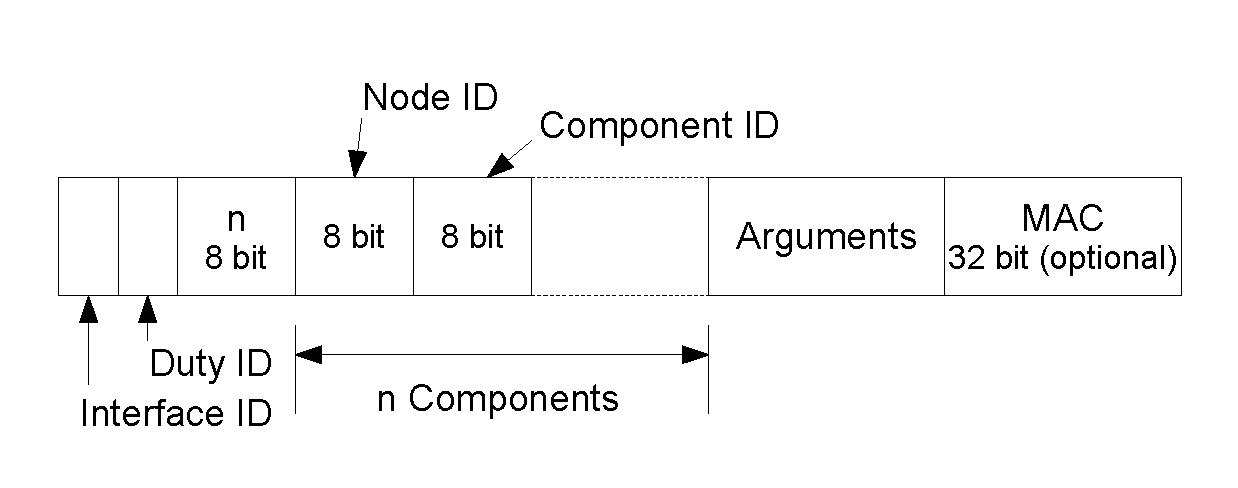
\includegraphics[scale=0.43]{packet}
  \caption{SpartanRPC data packet format.}
  \label{fig:packet}
\end{figure}

The SpartanRPC packet header can introduce significant overhead in some cases. In the current
version of Sprocket, $I$ and $D$ are packed as two four bit fields in a single byte. Each
intended destination is identified by a byte for $N$ and a byte for $C$. Finally an additional
byte is used to encode the header's size. This yields a total overhead of $2 + 2n$ bytes where
$n$ is the number of components intended to receive the packet. A special node ID of \code{0xFF}
is used to represent a SpartanRPC level broadcast. Thus in the special (and common) case where
all neighbor nodes are to process the remote call the overhead is exactly four bytes, leaving 12
bytes for duty parameters. If a parameterless duty is called, the maximum fan out supported by
our implementation is seven.

The limited field sizes used in the header put static restrictions on the system. Only 16 remote
interfaces per component can be used with at most 16 duties per interface. In addition, the
current version of Sprocket limits the network to at most 255 nodes with 256 remotely accessible
components per node.

\subsection{Skeleton Generation}

For each remote interface provided, Sprocket converts the duties in the component providing that
interface into nesC commands. Sprocket also generates a skeleton component for every remote
interface implementation. These skeletons are connected to the active message components in the
TinyOS library. Each time a duty message is received the skeleton checks the packet for
applicability. If the packet is not intended for the $(N, C, I)$ triple supported by the
skeleton or if $D$ is out of bounds for the interface, the packet is ignored. In the interest of
minimizing radio traffic, no error indication is returned.

If the packet is applicable, the skeleton unmarshalls the message, stores the duty arguments in
skeleton-local variables, and posts a task that implements the duty. For each duty in the
provided interface, Sprocket generates a trivial task in the skeleton that simply calls the
converted duty. For example:
\begin{Verbatim}
// 'value' written when packet unmarshalled.
uint8_t value;
task void setLeds()
    { call Blink.setLeds(value); }
\end{Verbatim}
\vspace{0.3em}

Thus the task-like semantics of duties are ultimately implemented in terms of ordinary nesC
tasks.

\subsection{Stub Generation}

On the RPC client side, Sprocket converts each duty posting into a command in a stub component
generated by Sprocket. That command first calls the \code{elements} command in the component
manager to obtain the list of target components. It then prepares a SpartanRPC data packet by
marshalling the duty arguments. Finally it broadcasts the packet to all neighboring nodes using
the TinyOS active message library. Recipients discern packets intended for them via packet
identifiers as described above.

Sprocket converts dynamic wires into static wiring that connects the posting component to the
generated stub. The stub is connected to the component manager associated with the dynamic
wiring. For example, a dynamic wire such as:
\begin{Verbatim}
ClientC.LEDControl ->
    [RemoteSelectorC].LEDControl;
\end{Verbatim}
is converted converted into the configuration as follows:
\begin{Verbatim}
components Spkt__1;
ClientC.LEDControl -> Spkt__1;
Spkt__1.ComponentManager -> RemoteSelectorC;
Spkt__1.Packet    -> AMSenderC;
Spkt__1.AMPacket  -> AMSenderC;
Spkt__1.AMControl -> ActiveMessageC;
Spkt__1.AMSend    -> AMSenderC;
\end{Verbatim}

The \code{Spkt\_\_1} component is the Sprocket generated stub.

\subsection{Security}

When capability-based security is used, Sprocket consults a configuration file that maps
capabilities to keys. To activate a capability over a dynamic wire, the Sprocket generated stub
computes a MAC that covers the SpartanRPC header and marshalled duty arguments. In the current
implementation this MAC is computed using the AES encryption algorithm in CBC mode with an
initialization vector of zero. Because SpartanRPC packets are currently limited to 16 bytes,
only a single AES encryption is necessary to compute the MAC. The first four bytes of the
resulting cipher text is used as the MAC value. While a MAC of only 32 bits would not normally
be considered secure, wireless sensor networks generate data so slowly that attacking even such
a short MAC is not considered feasible \cite{karlog-tinysec-2004,luk-minisec-2007}. Our MAC
computation is simplistic, but we feel it is adequate to demonstrate a proof of concept.

For components providing a secure remote interface, the generated skeleton incorporates a MAC
authentication procedure under the required key as declared in the component specification. The
usual checks of interface ID and component ID are done first so as to avoid a costly MAC
computation in the case where the received packet is not actually intended for the skeleton.
Only when the other applicability checks succeed is the MAC checked. The duty invocation is
ignored if the MAC check fails.

\section{Empirical Analysis of Overhead}
\label{sec:empirical-results}
\label{section-empirical-results}

The practicality of our system depends on its cost in terms of memory
and processor overhead. In this section we report on performance
measurements made on our implementation. In summary, we show that our
combined use of public and private key cryptography in the underlying
security protocol imposes a low amortized cost over time, despite high
costs for initial authorizations.

\paragraph{Test Environment and Programs.} Since many communication
chips now support hardware AES encryption, we were primarily interested
in demonstrating performance using that feature. In particular, the
popular MEMSIC TelosB wireless sensor mote \cite{telosb-datasheet} uses
a Chipcon CC2420 transceiver with hardware encryption. Unfortunately,
the standard TOSSIM simulation environment does not model hardware
encryption for TinyOS 2.1, so all of our tests were performed on real
hardware. We used TelosB motes, with 10\,KB of RAM, 48\,KB of ROM and an
8\,MHz MSP430 microcontroller running TinyOS 2.1.2 \cite{tinyos}.

We exercised our system using both small test programs and using our
implementation of the directed diffusion example described in
\autoref{section-example}. The small test programs consisted of a simple
client/server pair where the client repeatedly sent a message containing
a single 16~bit value to the server. The purpose of these tests was to
explore the overhead induced by our system with minimal obscuring
effects from application logic. The percentage overhead observed with
the small programs is thus a worst case overhead. In contrast, the
directed diffusion example allowed us to test the behavior of the system
in a more realistic, long-running setting. It serves as a demonstration
that our system is feasible in practice, and allowed us to exercise our
system in a multi-mote, multi-hop network environment.

\subsection{Memory Overhead for Security Features}

The \Sprocket\ run time system uses several memory caches to hold key
material, credential information, and the minimum model implied by the
set of known credentials. These caches are statically allocated but must
be stored in RAM since their contents are dynamic.
Table~\ref{table-ram-consumed} summarizes the RAM consumption of the
various storage areas used by the current implementation.

\begin{table}[!t]
  \newcommand\T{\rule{0pt}{2.1ex}}
  \centering
  \tbl{RAM consumed by various storage areas}
  {
  \begin{tabular}{|l|r|r|r|} \hline
    \textit{Storage Area} \T & \textit{\# Items} & \textit{Bytes/Item} & \textit{Total Bytes} \\
    \hline \hline

    Session Keys ($n_k$) \T & 10 & 22 & 220 \\ \hline 
    Public Keys ($n_p$)  \T & 12 & 40 & 480 \\ \hline
    Credentials ($n_c$ ) \T & 12 & 16 & 192 \\ \hline
    Model ($n_m$)        \T & 16 &  6 &  96 \\ \hline \hline
    \textbf{Total} \T & \multicolumn{3}{r|}{ \textbf{988} } \\ \hline
  \end{tabular}
  }
  \label{table-ram-consumed}
\end{table}

The number of items in each cache are tunable parameters. The optimum
settings depend on the intended application. The values in
Table~\ref{table-ram-consumed} attempt to strike a balance between
usability and flexibility on one hand and excessive memory consumption
on the other. In applications where these needs are more clearly known a
priori, the sizes of the caches can be adjusted to potentially result in
lower memory consumption.

Table~\ref{table-test-program-ram} shows the overall memory consumption
of two small client/server pairs. The baseline pair handle all
communication through normal Active Message packets that are explicitly
programmed by the user. The SpartanRPC pair uses our system which
includes support for certificate distribution and verification, session
key management, authorization logic, and MAC computations.

\begin{table}[!t]
  \newcommand\T{\rule{0pt}{2.1ex}}
  \centering
  \tbl{Memory consumption of test programs}
  {
  \begin{tabular}{|l|r|r|} \hline
    \textit{Test Program} \T & \textit{RAM Bytes} & \textit{ROM Bytes} \\
    \hline \hline

    Baseline Client   \T &  349 & 10982 \\ \hline 
    Baseline Server   \T &  283 & 10490 \\ \hline
    SpartanRPC Client \T & 2222 & 23108 \\ \hline
    SpartanRPC Server \T & 2126 & 23394 \\ \hline
  \end{tabular}
  }
  \label{table-test-program-ram}
\end{table}

Although the overhead incurred by the \Sprocket\ runtime system is
significant on our test platform, nearly 80\% of RAM and 50\% of ROM
resources are still available. Furthermore, these memory usage numbers
scale to denser neighborhoods and extended RPC services.

% The directed diffusion application consumes 27826 bytes of ROM and
% 3105 bytes of RAM.

\subsection{Transient and Steady State Processor Overhead} 

The execution performance of our system displays two distinct behaviors.
The first is a transient behavior that occurs after a node boots when
certificates are exchanged and session keys are negotiated between the
new node and its neighbors. The second is a steady-state behavior that
occurs during normal operation. The transient overhead of our system is
large but the steady state overhead is not. In a quasi-static
environment where new nodes enter the network infrequently the transient
costs are amortized and it is the small, steady state overhead that
dominates.

To explore the steady state overhead three tests were conducted.
\begin{longenum}
\item A baseline test where the message handling was done explicitly
  using traditional Active Message interfaces.
\item A duties test where the \Sprocket\ system was used but no
  authorization was requested. This is equivalent to using the
  authorization components \texttt{ACNullC} and \texttt{ASNullC} in
  \autoref{figure-client-server-authorization}.
\item A MAC test where authorization was requested but where the session
  key storage areas were preloaded with appropriate session keys.
\end{longenum}

Table~\ref{table-steady-state} shows the maximum rate at which messages
could be sent and received by the test programs mentioned above. Note
that the MAC test made use of the hardware assisted AES support provided
by the CC2420 radio chip. These results show that maximum message send
rates decrease by a factor of 7\% due to the addition of our duties
program logic (our security API), and further decreases by a factor of
25\% due to MAC calculations. We note that the latter overhead would be
incurred in any system using CC2420 MAC calculations.

\begin{table}[!t]
  \newcommand\T{\rule{0pt}{2.1ex}}
  \centering
  \tbl{Maximum message transfer rate}
  {
  \begin{tabular}{|l|r|r|} \hline
    \textit{Test} \T & \textit{messages/s} & \textit{\% Reduction} \\
    \hline \hline

    Baseline \T & 128 &   -- \\ \hline 
    Duties   \T & 119 &  7.0 \\ \hline
    MAC      \T &  87 & 32.0 \\ \hline
  \end{tabular}
  }
  \label{table-steady-state}
\end{table}

The transient runtime overhead of our system can be subdivided into
three primitive operations: the time required to transmit and verify a
certificate, the time required to build the minimum model, and the time
required to negotiate a session key. Two of these operations require
lengthy public key computations and dominate the transient behavior of
our system. Thus the performance of our system in this regard is closely
tied to the performance provided by TinyECC, which we used with default
settings (no optimizations). Table~\ref{table-transient-time} shows the
times required for each of the primitive transient operations in our
implementation.

% TinyECC provides a number of tunable parameters that can be used to
% optimize performance by trading off space and time
% \cite{Liu-Peng-TinyECC-2008}. In our tests, since we had no particular
% application constraints in mind, we used the TinyECC ``out of the
% box.'' However, TinyECC's optimizations can be used to tune the
% performance of our system to better match a particular application.
% For example, activating the Shamir Trick cut certificate verification
% time in half at the expense of increasing RAM usage by nearly 700
% bytes.

\begin{table}[tbhp]
  \newcommand\T{\rule{0pt}{2.1ex}}
  \centering
  \tbl{Transient processing time}
  {
  \begin{tabular}{|l|r|} \hline
    \textit{Operation} \T & \textit{Time} \\ \hline \hline

    Certificate Verification     \T &  82s \\ \hline 
    Minimum Model Construction   \T & 370$\mu$s \\ \hline
    Session Key Negotiation      \T &  80s\\ \hline
  \end{tabular}
  }
  \label{table-transient-time}
\end{table}

The time required to build the minimum model is directly related to the
number and nature of the credentials involved. In our test we used a
collection of five representative credentials, one of each type. In any
case this time is entirely negligible compared to the other transient
operations.

% There might be a termination problem with my algorithm for updating
% the minimum model despite the fact that the method I'm using is
% theoretically guaranteed to terminate. In particular if the model is
% too large it might be possible for the algorithm to run infinitely,
% alternating between replacing two different tuples in the limited
% space.

The time quoted for session key negotiation represents the time required
for both negotiating partners to compute the session key. In the current
implementation the two negotiating nodes do this sequentially with the
server node computing the session key before responding to the client
node. This was done in case the session key computation failed on the
server to ensure that the client does not falsely believe a session key
was successfully negotiated.

\subsection{Transient State Times for Directed Diffusion}

As argued above, the overhead imposed by our system is primarily the
time the network spends in a initial transient state when credentials
are verified and session keys are negotiated. Subsequently, the network
enters a steady state during which the main cost is a 32\% reduction in
\emph{maximal} message send rates due to hardware MAC computation. In
order to evaluate the performance of our system in a realistic
application, we therefore quantified the transient state times of the
secure directed diffusion application described in
\autoref{section-example}. In our experiments we elected a single node
to repeatedly express an interest and we observed how long was required
for that interest to flood the network. This time depends on three major
factors:
\begin{enumerate}
\item The number of certificates transferred.
\item The number of neighbors for each node.
\item The number of hops to the ``far'' edge of the network.
\end{enumerate}
We conducted two experiments, one on a single hop (star) network and 
another on a multi-hop (mesh) network.

In the single hop case, transient time $T$ can be described by the
following equation:

\begin{displaymath}
T = n_c B + V + n_n K
\end{displaymath}

where $B$ is the certificate broadcast interval, $V$ is the certificate
verification time, $K$ is the session key negotiation time, $n_c$ is the
number of certificates and $n_n$ is the number of neighbors. Since $B$
was set to 90 seconds, which is greater than $V$, certificate
verification for $n_c$ certificates takes time $n_c B + V$ given a 90
second system initialization period. And since session keys need to be
negotiated with $n_k$ neighbors in turn, $T$ also comprises a $n_nK$
delay. Table~\ref{table-one-hop-transient} shows the transient time
required to flood a network where all nodes are one-hop neighbors of the
root node. Values are given for three different policies with different
numbers of certificates transferred from the root to the neighbors.

\begin{table}[tbhp]
  \newcommand\T{\rule{0pt}{2.1ex}}
  %\tbl{}%Transient time in directed diffusion}
  {
  \begin{minipage}{.5\linewidth}
    \centering
    \tbl{Single hop transient time}
    {
    \begin{tabular}{|l|r|r|r|} \hline
      \textit{\# neighbors} \T & \textit{1 Cert }
                               & \textit{2 Certs}
                               & \textit{3 Certs} \\ \hline \hline

      1 \T &  4m03s & 5m27s &  6m52s \\ \hline
      2 \T &  5m16s & 6m50s &  8m24s \\ \hline
      3 \T &  6m32s & 7m57s &  9m30s \\ \hline
      4 \T &  7m50s & 9m22s & 10m51s \\ \hline
    \end{tabular}
    }
    \label{table-one-hop-transient}
  \end{minipage}%
  \begin{minipage}{.5\linewidth}
    \centering
    \tbl{Multi-hop transient time}
    {
    \begin{tabular}{|l|r|r|r|} \hline
      \textit{Run} \T & \textit{1 hop }
                      & \textit{2 hops}
                      & \textit{3 hops} \\ \hline \hline

      1 \T &  4m05s & 7m24s & 9m10s \\ \hline
      2 \T &  3m12s & 5m12s & 6m30s \\ \hline
      3 \T &  3m57s & 7m37s & 9m15s \\ \hline
      4 \T &  4m09s & 7m15s & 8m49s \\ \hline
      \textit{Average} \T &  3m51s & 6m52s & 8m23s \\ \hline
    \end{tabular}
    }
    \label{table-multi-hop-transient}
  \end{minipage}
  }
\end{table}

We explored the behavior of our system in a multi-hop environment by
creating a linear mesh network. Each node (except the root) had a single
downstream neighbor. All nodes were booted simultaneously and the time
required for interest information to reach each node was observed. The
policy used required only a single certificate to be transferred between
nodes. Table~\ref{table-multi-hop-transient} shows the results of
several runs.

The reason for variations in transient times over each run was due to a
randomized element in the protocol, specifically a randomized $\pm 10\%$
interval in certificate broadcast times to avoid collisions. In these
results it is essential to note that for hops $> 2$, extra transient
time is comprised solely of session key negotiation times (80s per
session key, see Table~\ref{table-transient-time}) that are forced by
duty postings as interests propagate through the network. Certificates
are broadcast and verified in parallel throughout the network upon
system boot up, during the same time period required for the root's
interest to propagate through the first and second hops.

\section{A Prototype Application}
\label{section-snowcloud}

To evaluate the performance of SpartanRPC in a real application
setting, we have used the system to implement secure versions of data
collection and sampling control protocols in an environmental
monitoring system. The Snowcloud system
\cite{frolik-skalka-snowcloudtr,moeser-walker-skalka-frolik-wsc11} is
a WSN developed at the University of Vermont for snow hydrology
research applications.  It is based on the MEMSIC TelosB mote platform
running TinyOS, and has seen multiple field deployments. Typical
deployed systems comprise 4-8 sensor nodes but the technology is
currently scalable to arbitrary numbers of nodes. For data collection
and sampling rate control, the system also includes a handheld
``Harvester'' device.  This device incorporates a TelosB mote to
establish a network connection when in radio communication with the
deployment.  Users transport the device to and from deployment sites,
and interact with the sensor node network by issuing commands from a
simple push-button interface. A Harvester device and a deployed
Snowcloud sensor tower are pictured in \autoref{figure-snowcloud}. The
scheme described here has been implemented and tested in our test
network at UVM, which uses the same software and hardware platforms as
in our active deployments.

\snowcloudfig

In our secured version of the Snowcloud system, the goal is to treat
data collection and sampling rate control as protected resources
requiring authorization. Furthermore, sampling rate modifications
should require a higher, ``administrator'' level of authorization than
data collection. That is, only system engineers should be able to
perform control operations, whereas data end-users making field visits
should be able to collect data.  Snowcloud sensor node code in
particular makes use of nearly every resource available on the mote--
including timing, sensor I/O, radio messaging, and flash memory, not
to mention CPU and main memory. Thus, it is a robust example of the
interaction of SpartanRPC with mote resources in real applications.

The system described here is also informative since it can be easily
ported to other similar application settings. That is, WSN application
settings wherein multiple users of various authorization levels need
to interact with the same network in control or collection capacities,
as mediated by security policy. The SpartanRPC API allows
straightforward retasking of authorized service implementations to
these various settings. Furthermore, the RT authorization logic
supports collaboration between multiple social domains, by allowing
security policy to be managed in a decentralized manner as we
illustrate below.

\subsection{Security Policies}

To specify and implement the security policies informally described
above, we consider the sensor network and the Harvester single node
``network'' as separate security domains, each with their own set of
credentials. The sensor network is always endowed with
administrator-level credentials. If a Harvester is to be used by a
system engineer, its mote is also endowed with administrator-level
credentials, whereas a Harvester to be used by a data end-user is only
endowed with user-level credentials. When a Harvester is introduced to
the sensor network, its resource accesses are mediated by its
authorization level. Since credentials are unforgeable, a user-level
Harvester can never be used for sensor network control even if it is
reprogrammed.

Sensor nodes within the network possess four credentials, as follows.
In these credentials the Snowcloud domain is abbreviated
$\mathit{SC}$. Authority to collect data and control sensors in the
network are governed by the roles $\mathit{SC.Col}$ and
$\mathit{SC.Con}$, respectively.  Credential (1) says that control
authority contains collection authority. (2) says that nodes in the
Snowcloud domain have control authority. (3) says that any entity in a
Snowcloud collaborator's $\mathit{Usr}$ role has collection
authority. (4) says that the node identified by $\mathit{NId}$ is in
the Snowcloud domain.
\begin{mathpar}
(1)\quad \cred{SC.Col}{SC.Con}

(2)\quad \cred{SC.Con}{SC.Node}

(3)\quad \cred{SC.Col}{SC.Collab.Usr}

(4)\quad \cred{SC.Node}{NId}
\end{mathpar}
When invoking remote services, the node will do so on behalf of the
entity $\mathit{NId}$. It will also be imaged with the $\mathit{NId}$
private key for session key negotiation.

Any Harvester within the Snowcloud domain is then provided with the
credential $\cred{SC.Node}{HId}$ and the $\mathit{HId}$ private key
issued by Snowcloud domain administration. This will provide that
Harvester with collection and control authority in the domain. For
Harvesters to be provided to collaborators, the Snowcloud
administrators issue a credential establishing the institution as a
collaborator, while the institution itself may define and manage policy
for their $\mathit{Usr}$ role membership. For example, the University
of New Hampshire ($\mathit{UNH}$) can be established as a collaborator
with credential (5) issued by Snowcloud domain administration, and may
specify role membership with the credential (6) issued by UNH domain
administration:
\begin{mathpar}
(5)\quad \cred{SC.Collab}{{UNH}}

(6)\quad \cred{{UNH}.Usr}{UsrID}
\end{mathpar}
These two credentials, along with the $\mathit{UsrID}$ private key,
are imaged on Harvesters issued to UNH collaborators for data
collection, but which remain unauthorized for control.

\subsection{Implementation}

Resources themselves are accessed through a secure command
dissemination protocol, that is modeled upon the TinyOS Dissemination
protocol (as described in TEP 118). In short, protected RPC services
establish network level broadcast channels requiring authorization for
use. Commands are communicated to the network over these channels, and
different channels are used for different sorts of commands. 

In more detail, command broadcast services can be specified as a duty
in a remotable interface:
\begin{Verbatim}[fontsize=\small]
    interface SpDisseminationUpdate { duty void change(command_t new_value); }
\end{Verbatim}
To implement e.g.~the control command channel, the following module
can be defined and included on sensor nodes in the Snowcloud domain:
\begin{Verbatim}[fontsize=\small]
    module ControlDissemC {
        provides remote interface SpDisseminationUpdate requires "SC.Con";
        uses            interface SpDisseminationUpdate as NeighborUpdate;
        provides        interface ComponentManager;
    }
    implementation { ... }
\end{Verbatim}
In the implementation, the provided $\verb+SpDisseminationUpdate+$
interface accepts command invocations from neighbors, but requires
them to be authorized for the $\mathit{SC.Con}$ role. Commands are
relayed to all other neighbors (i.e.~disseminated) via the used
$\verb+NeighborUpdate+$ interface; those neighbors are identified by
the provided $\verb+ComponentManager+$.

To use this component, both sensor and Harvester nodes can configure 
it through the following component instantiation and wiring, where 
the component's $\verb+NeighborUpdate+$ interface is wired remotely
to neighbors: 
\begin{Verbatim}[fontsize=\small]
    components ControlDissemC as ControlChan;
    activate "*" for 
        ControlChan.NeighborUpdate -> [ControlChan].SpDisseminationUpdate;
\end{Verbatim}
Note that a node must be endowed with the appropriate credentials for
this wiring to be useful. 

This same code pattern can be used to implement a data collection
request channel, protected by the $\mathit{SC.Col}$ role instead of
$\mathit{SC.Con}$. In response to an authorized control command
invocation, sensor nodes will modify their behavior appropriately,
whereas in response to authorized data collection requests sensor
nodes will report their data using collection tree protocol (TEP 123)
to the Harvester.

Note that since the only ``border'' between security domains in this
scenario is between the Harvester and its neighbor(s), Snowcloud
scalability is not affected. Only authorization between the Harvester
and its one-hop neighbors needs to be established no matter what the
network size, and since areal coverage is the goal of a deployment,
network densities remain fairly constant where neighborhoods are on
the order of 1-5 nodes in conceivable deployments.

\subsection{Results}

Results can be characterized according to both the application
end-user experience and to quantitative aspects. As detailed in
\autoref{section-empirical-results}, a one-time transient overhead is
imposed for initial credential exchange and session key negotiation
when a Harvester is first introduced to the network. However, since
data collection for a network after several months of deployment can
take up to an hour, this overhead is relatively insignificant. And
steady-state overhead is small, and does not affect data collection
rates. Further, subsequent field visits will not impose transient
overhead since negotiated keys can be cached in non-volatile
memory. Thus, authorized user experience is not significantly impacted
by the addition of security.

From a quantitative perspective, the most important measurements to
consider for this application, beyond the general ones already
considered in \autoref{section-empirical-results}, are RAM and ROM
consumption of the insecure and secured versions of the Harvester
collection protocol. We have to consider whether layering SpartanRPC
security over a realistic application will overrun the resources
available to a mote platform. Relevant measurements are as follows.
\begin{table}[h]
\centering \newcommand\T{\rule{0pt}{2.1ex}}
  \tbl{RAM and ROM use for Snowcloud versions}
  {
  \begin{tabular}{|l|c|c|} \hline
    \emph{Program}       \T & \emph{RAM Bytes} & \emph{ROM Bytes} \\ \hline\hline
    Insecure Harvester   \T & 2274             & 24316 \\ \hline
    Secure Harvester     \T & 4771             & 35834 \\ \hline
    Insecure Sensor Node \T & 2868             & 36254 \\ \hline
    Secure Sensor Node   \T & 5417             & 48616 \\ \hline
  \end{tabular}
  }
  \label{table-snowcloud}
\end{table}

Both RAM and ROM consumption are significantly increased by the addition
of SpartanRPC security to this application. However, these numbers are
within operating parameters, and the Sprocket implementation of
SpartanRPC described in \autoref{section-implementation} has not yet
been optimized for space efficiency in any way; improvements in this
respect can be made but are out of scope for this work.

\section{Related Work}
\label{section-related-work}

Extending wireless sensor network software platforms with support for
secure interactions between domains has been studied in previous
research on SSL for WSNs \cite{10.1109/WAINA.2009.47}. However, this
work was focused on extending the Internet to WSNs (a.k.a. ``IP for
WSNs''), whereas SpartanRPC is a more general system for enhancing
secure communications \emph{within} a WSN.  Research on WSN security
has also addressed secure routing \cite{senroute-ahnj03}, link layer
security \cite{karlog-tinysec-2004}, cryptography \cite{bertoni-2006},
key distribution \cite{camtepe-bulent-05}, and hardware issues
\cite{perrig-2004}. In contrast to these low-level systems, SpartanRPC
provides language-level abstractions for secure RPC services.  Perhaps
even more closely related in this same vein is a system for
establishing fine-grained, ``node-level'' policies in WSNs
\cite{Claycomb:2011:NNL:1889383.1889450}. However, this work is more
focused on group-based key negotiation and distribution, and while it
does offer a policy language, it is rooted in implementation details
and not a separable specification as in our system. Also, they do not
provide a language API for integrating their system into secure
applications as in SpartanRPC.

Previous related work also illustrates interest in and useful
applications of RPC in embedded networks. For example, the Marionette
system uses network layer RPC for remote (PC-based) analysis and
debugging of WSNs \cite{whitehouse-marionette-2006}. The Fleck operating
system provides a small pre-defined set of RPC services for WSN
applications, while the trustedFleck system extends this with a form a
secure RPC \cite{hu-secfleck-2009,Hu:2010:TTW:1806895.1806900}. S-RPC
provides an RPC facility for sensor networks that allows remote services
to be added to the system dynamically \cite{5766863}. SpartanRPC differs
from these systems in that it extends the nesC programming language
(unlike trustedFleck) to allow programmer definition of secure RPC
services (unlike S-RPC) that can be accessed by nodes within the network
itself (unlike Marionette). Our system is similar to and inspired by
TinyRPC \cite{may-tinyrpc-2007}, except the latter does not provide
security and has a different semantics that are not as expressive as our
approach.


Teeny\textsc{lime} allows application programs to access an abstract
``tuple space'' that is the union of tuple spaces on the local node and
the immediately neighboring nodes \cite{Costa:2007:PWS:1516124.1516153}.
This provides an alternative to RPC for uniformly accessing remote and
local data. However, interaction with the middleware is by way of a
dedicated API; there is no attempt to provide a true RPC mechanism. Also
Teeny\textsc{lime} does not address issues of access control.

Secure Middleware for Embedded Peer to Peer systems (SMEPP) is a general
framework for creating security sensitive applications from a
distributed network of embedded peers
\cite{Brogi:2008:SME:1363370.1363548}. SMEPP Light
\cite{Vairo:2008:SMW:1594978.1595054} is a reduced version of SMEPP to
address the resource constraints of wireless sensor networks. SMEPP
Light provides a publish/subscribe communication model using directed
diffusion to distribute ``events'' to all subscribers and symmetric key
cryptography to provide confidentiality and data integrity within a
group of nodes. However, SMEPP Light is not integrated into a
programming language and does not provide a remote procedure call
mechanism. Furthermore SMEPP Light only supports a simple model of
access control based on group membership.

High level macro\-programming languages such as Kairos
\cite{springerlink:10.1007/1150259312}, Regiment
\cite{Newton:2007:RMS:1236360.1236422}, and even Flask
\cite{Mainland-Flask-2008} provide a way to program the entire network
as a single entity. These systems attempt to hide not only the
inter-node communication from the programmer, but also the entire node
level programs. SpartanRPC operates at a much lower level and also,
unlike these macro\-programming systems, addresses access control issues
in networks containing multiple security domains.

Whole network programming of wireless sensor networks has also been
investigated using mobile agents in systems such as Agilla
\cite{Fok:2009:AMA:1552297.1552299} and Wiseman
\cite{Gonzalez-Valenzuela:2010:PMW:1891545.1891566}. However, like the
macro\-programming systems mentioned previously neither of these systems
address issues related to access control in the presence of multiple
security domains.

\section{Conclusion}
\label{section-conclusion}

We have designed and implemented SpartanRPC, a dialect of nesC with a
light weight, link-layer, secure RPC API. SpartanRPC is a middleware
technology supporting secure WSN applications comprising multiple
security domains. It is ideal for settings in which multiple networks
administered by distinct social entities cooperate to obtain a
holistic behavior. As discussed in \autoref{section-related-work},
currently no other WSN security architectures support multiple
security domains or principled techniques for communication between
them. Thus, SpartanRPC provides crucial tools for next-generation WSN
applications wherein multiple, distinct security domains interact.

RPC communication in our system is implemented using a modification of
existing nesC abstractions, specifically module wirings. In
SpartanRPC, module wirings connect to remote services dynamically.
Furthermore, these connections are mediated by authorization levels
specified by an access control policy defined in the trust management
language RT \cite{Li:DRBTMF}, and authorization is proved by
presentation of RT credentials by requesters. Our implementation is
based on public keys, supporting an open-world security model where
shared secrets need not be known a priori. Underlying security
protocols defend against man-in-the middle attacks through the use of
a Diffie-Hellman protocol, ensuring that only authorized principals
may access resources. We have reported on testing and performance
evaluations, providing evidence of the practicality of SpartanRPC in
its intended application space.  We have also used SpartanRPC to
implement a secure real-world WSN application for environmental data
collection, demonstrating the effectiveness of the API and of the
authorization logic.


% ------------------------------
% Appendix and related materials
% ------------------------------

\bibliographystyle{ACM-Reference-Format-Journals}
\renewcommand{\showDOI}[1]{\unskip}
\bibliography{references-AccessControl,references-Meta,references-Security,references-WSN}

% History dates
\received{Month Year}{Month Year}{Month Year}

\end{document}
